\documentclass[aspectratio=169]{beamer}
\setbeamertemplate{navigation symbols}{}
\usepackage{color, amsmath, comment, subfigure}
\usepackage{url}

\usepackage{hyperref}
\hypersetup{
    colorlinks=true,
    linkcolor=blue,
    filecolor=magenta,      
    urlcolor=cyan,
}

%%%%%%%%%%%%%%%%%%%%%%%%%%
\title[]{Pre-read for Thursday, November 5:\\Disease empirics}
\author[]{Matthew J. Salganik}
\institute[]{}
\date[]{COS 597E/SOC 555 Limits to prediction\\Fall 2020, Princeton University}

\begin{document}
%%%%%%%%%%%%%%%%%%%%%%%%%%%
\frame{\titlepage}
%%%%%%%%%%%%%%%%%%%%%%%%%%%
\begin{frame}

\begin{columns}[c]
  \column{.5\textwidth}
  \begin{center}
  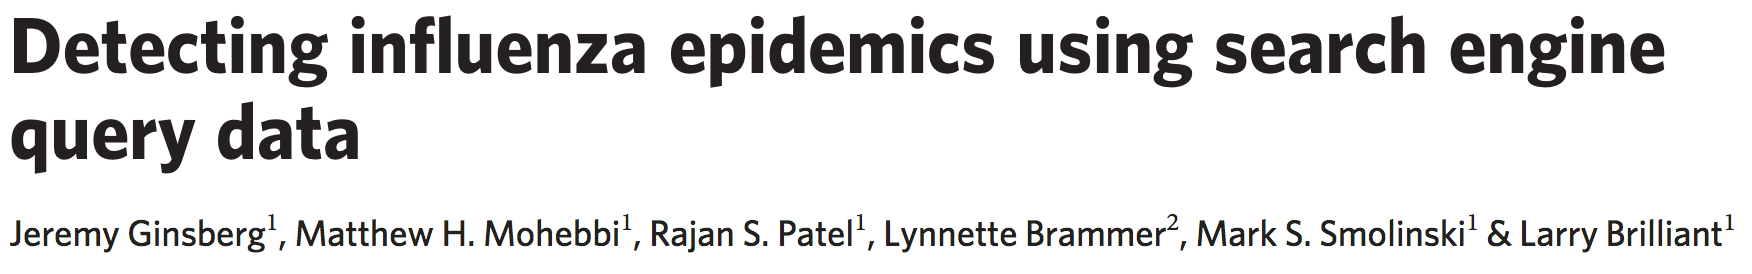
\includegraphics[width = 0.9\textwidth]{figures/ginsberg_detecting_2009_title}
  \end{center}
   \column{.5\textwidth} 
   \begin{center}
  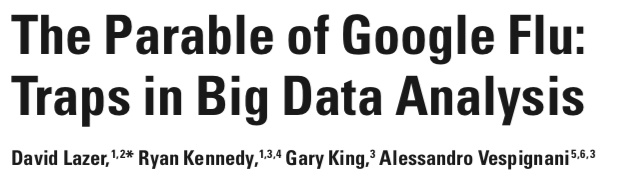
\includegraphics[width = 0.9\textwidth]{figures/lazer_parable_2014_title}
  \end{center}
\end{columns}

\end{frame}
%%%%%%%%%%%%%%%%%%%%%%%%%%%%%
\begin{frame}

\begin{center}
\begin{tabular}{ccc}
\onslide<1->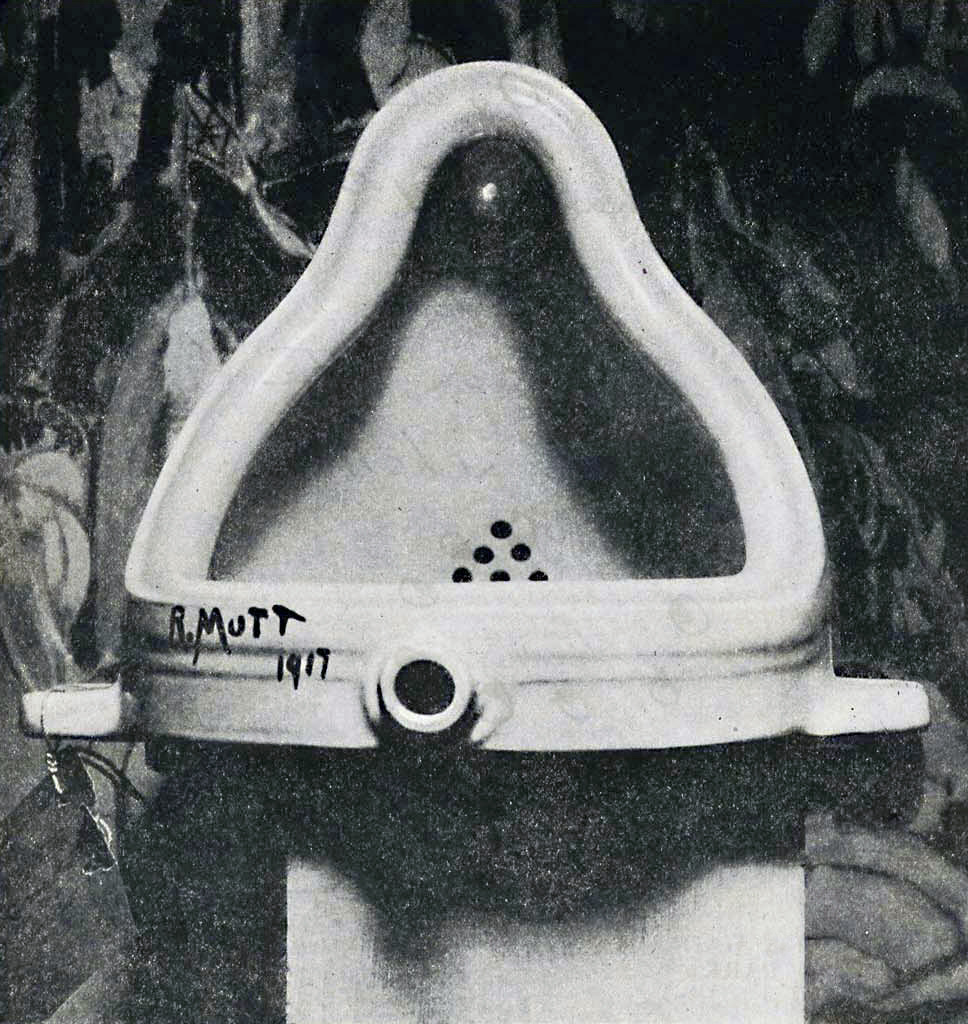
\includegraphics[width=0.30\textwidth]{figures/duchamp_fountain} & \phantom{12345} & \onslide<1->{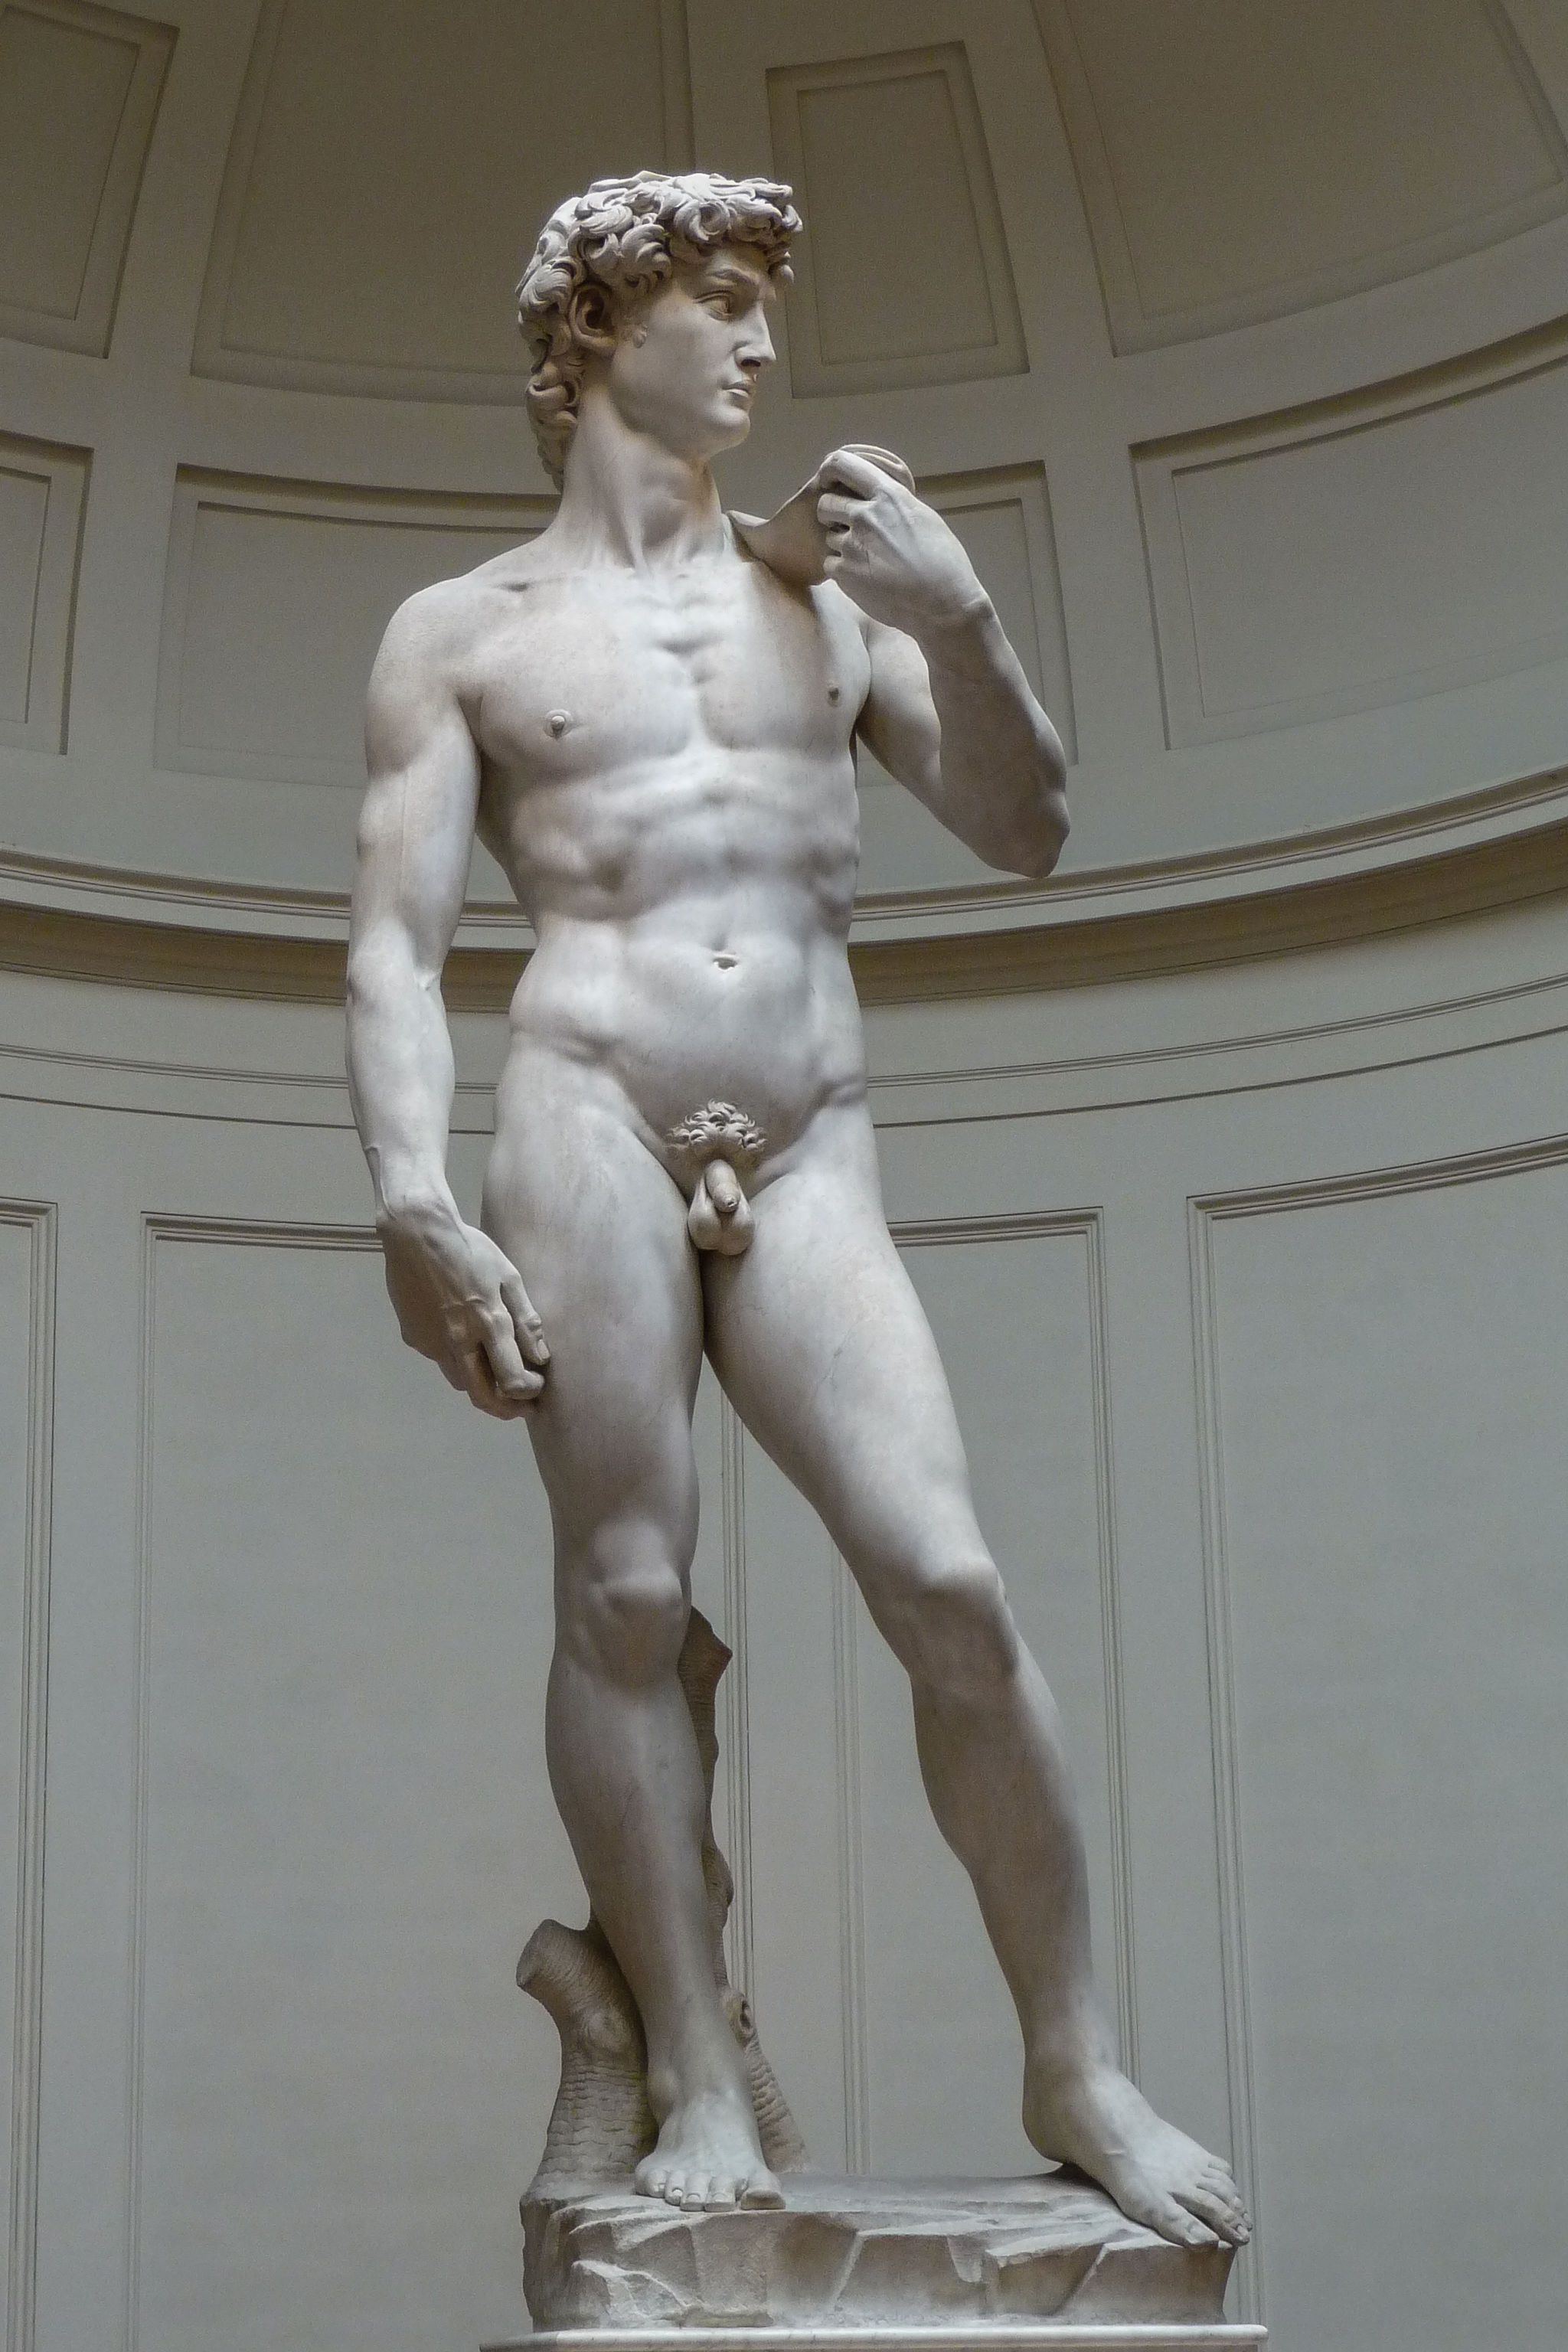
\includegraphics[width=0.30\textwidth]{figures/michelangelo_david}} \\
\onslide<1->{\LARGE{readymades}} &  & \onslide<1>{\LARGE{custommades}}
\end{tabular}
\end{center}

\vfill
\onslide<1>{
\TINY{\url{https://commons.wikimedia.org/wiki/File:Duchamp_Fountaine.jpg}}\\
\TINY{\url{https://commons.wikimedia.org/wiki/File:\%27David\%27_by_Michelangelo_JBU0001.JPG}}}

\end{frame}
%%%%%%%%%%%%%%%%%%%%%%%%%%%%
\begin{frame}

Reading notes:
\begin{itemize}
\item As you are reading the paper about Google Flu Trends, try to anticipate how it might go wrong and make a list.
\pause
\item After you read Lazer et al.\ see how your guesses compare to what they argue.
\pause
\item Do you think the problems with Google Flu Trends are fixable or fundamental? Does the fact that Google Flu Trends is now discontinued change your guess?
\end{itemize}

\end{frame}
%%%%%%%%%%%%%%%%%%%%%%%%%%%%%
\begin{frame}

Predicting the present vs predicting the future, but which is more important?

\end{frame}
%%%%%%%%%%%%%%%%%%%%%%%%%%%%%
\begin{frame}

\begin{center}
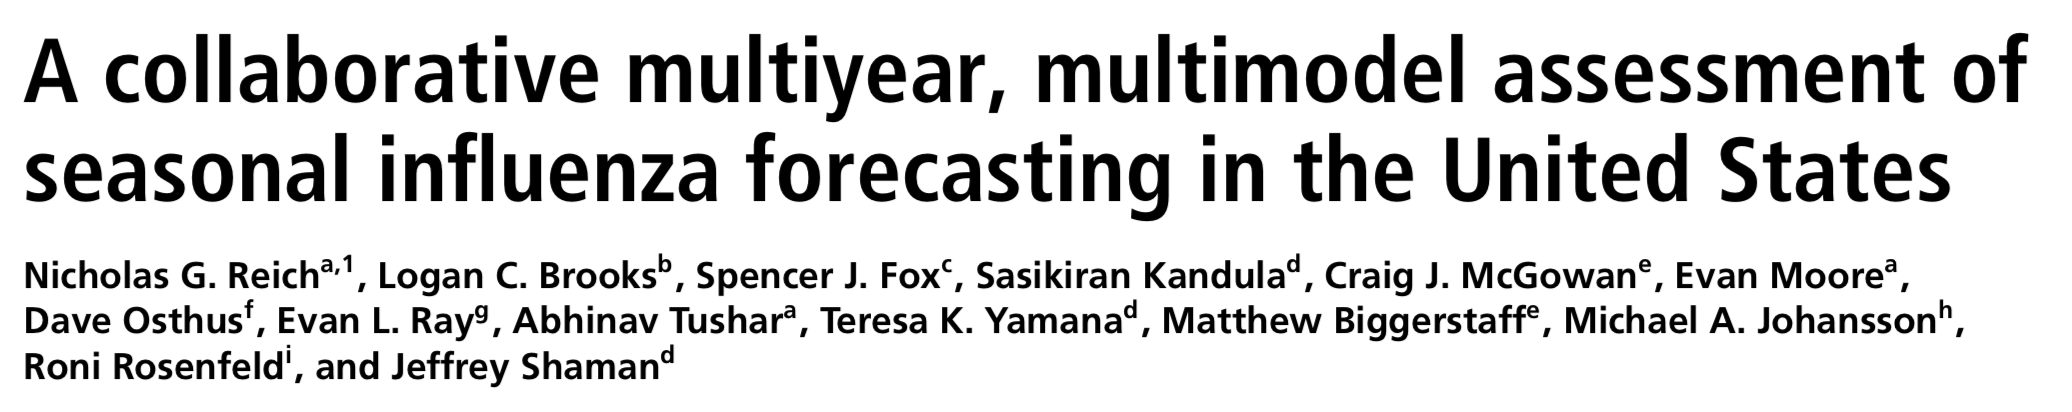
\includegraphics[width = 0.9\textwidth]{figures/reich_collaborative_2019_title}
\end{center}

\end{frame}
%%%%%%%%%%%%%%%%%%%%%%%%%%%%%%%
\begin{frame}

\begin{center}
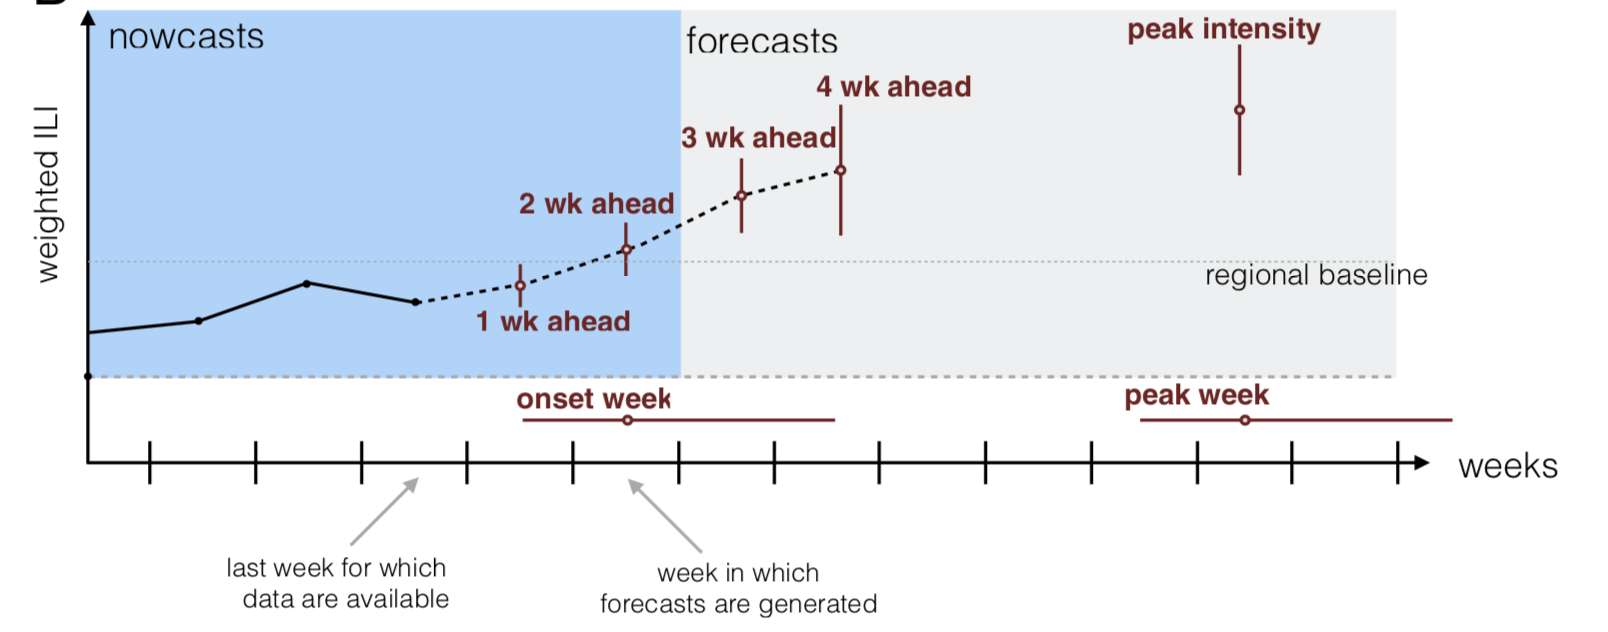
\includegraphics[width = 0.9\textwidth]{figures/reich_collaborative_2019_fig2b}
\end{center}

\end{frame}
%%%%%%%%%%%%%%%%%%%%%%%%%%%%%
\begin{frame}

Predictions are evaluated using (modified) log score.

Here are some predictions from the ReichLab-KDE model (the baseline model).

\begin{center}
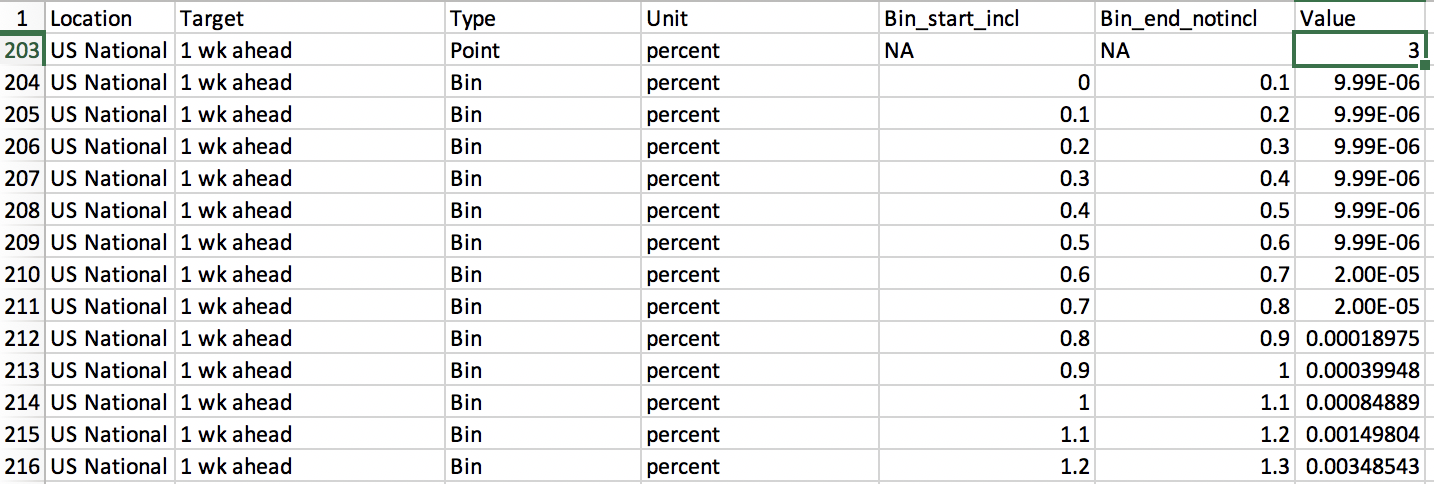
\includegraphics[width = 0.9\textwidth]{figures/reich_collaborative_2019_example_predictions}
\end{center}

If the true ILI\% was between 1.2 and 1.3 percent, then this model would get $ln(0.00348543)$.  You get more points putting on your probability weight on what happened.\\

\pause
CDC uses modified version of log score so that you get you get full credit if you with 0.5 percentage points.

\end{frame}
%%%%%%%%%%%%%%%%%%%%%%%%%%%%%
\begin{frame}

Reading notes:
\begin{itemize}
\item How does this relate to the common task method (e.g., ImageNet, Netflix Prize, Fragile Families Challenge)?
\pause
\item They are trying to predict the percentage of doctor visits that are related to influenza-like illness. How might this impact which kinds of approaches (statistical vs compartmental/mechanistic) are more or less effective?
\pause
\item How does the debate about what scoring metric to use recall some of the debates that we had on October 15?
\end{itemize}

\end{frame}
%%%%%%%%%%%%%%%%%%%%%%%%%%%%%
\begin{frame}

\begin{center}
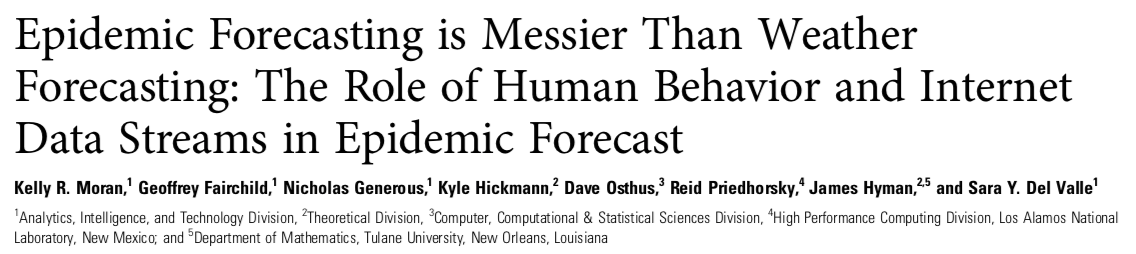
\includegraphics[width = 0.9\textwidth]{figures/moran_epidemic_2016_title}
\end{center}

\end{frame}
%%%%%%%%%%%%%%%%%%%%%%%%%%%%%
\begin{frame}

From class on October 24\\
The following conditions make prediction easier for weather than many of the others domains we have studied in the past:
\begin{itemize}
\item Many groups make public predictions every day at multiple time scales (5-day forecast, 10-day forecast), and we can all see how accurate they are
\pause
\item No self-fulfilling or self-defeating processes 
\pause
\item No concerns about causality
\pause
\item Predictions based a real physical model
\pause
\item Business and governments invests in improved performance
\end{itemize}

So even though this system is fundamentally unpredictable it has a lot going for it.

\end{frame}
%%%%%%%%%%%%%%%%%%%%%%%%%%%%%
\begin{frame}

\begin{center}
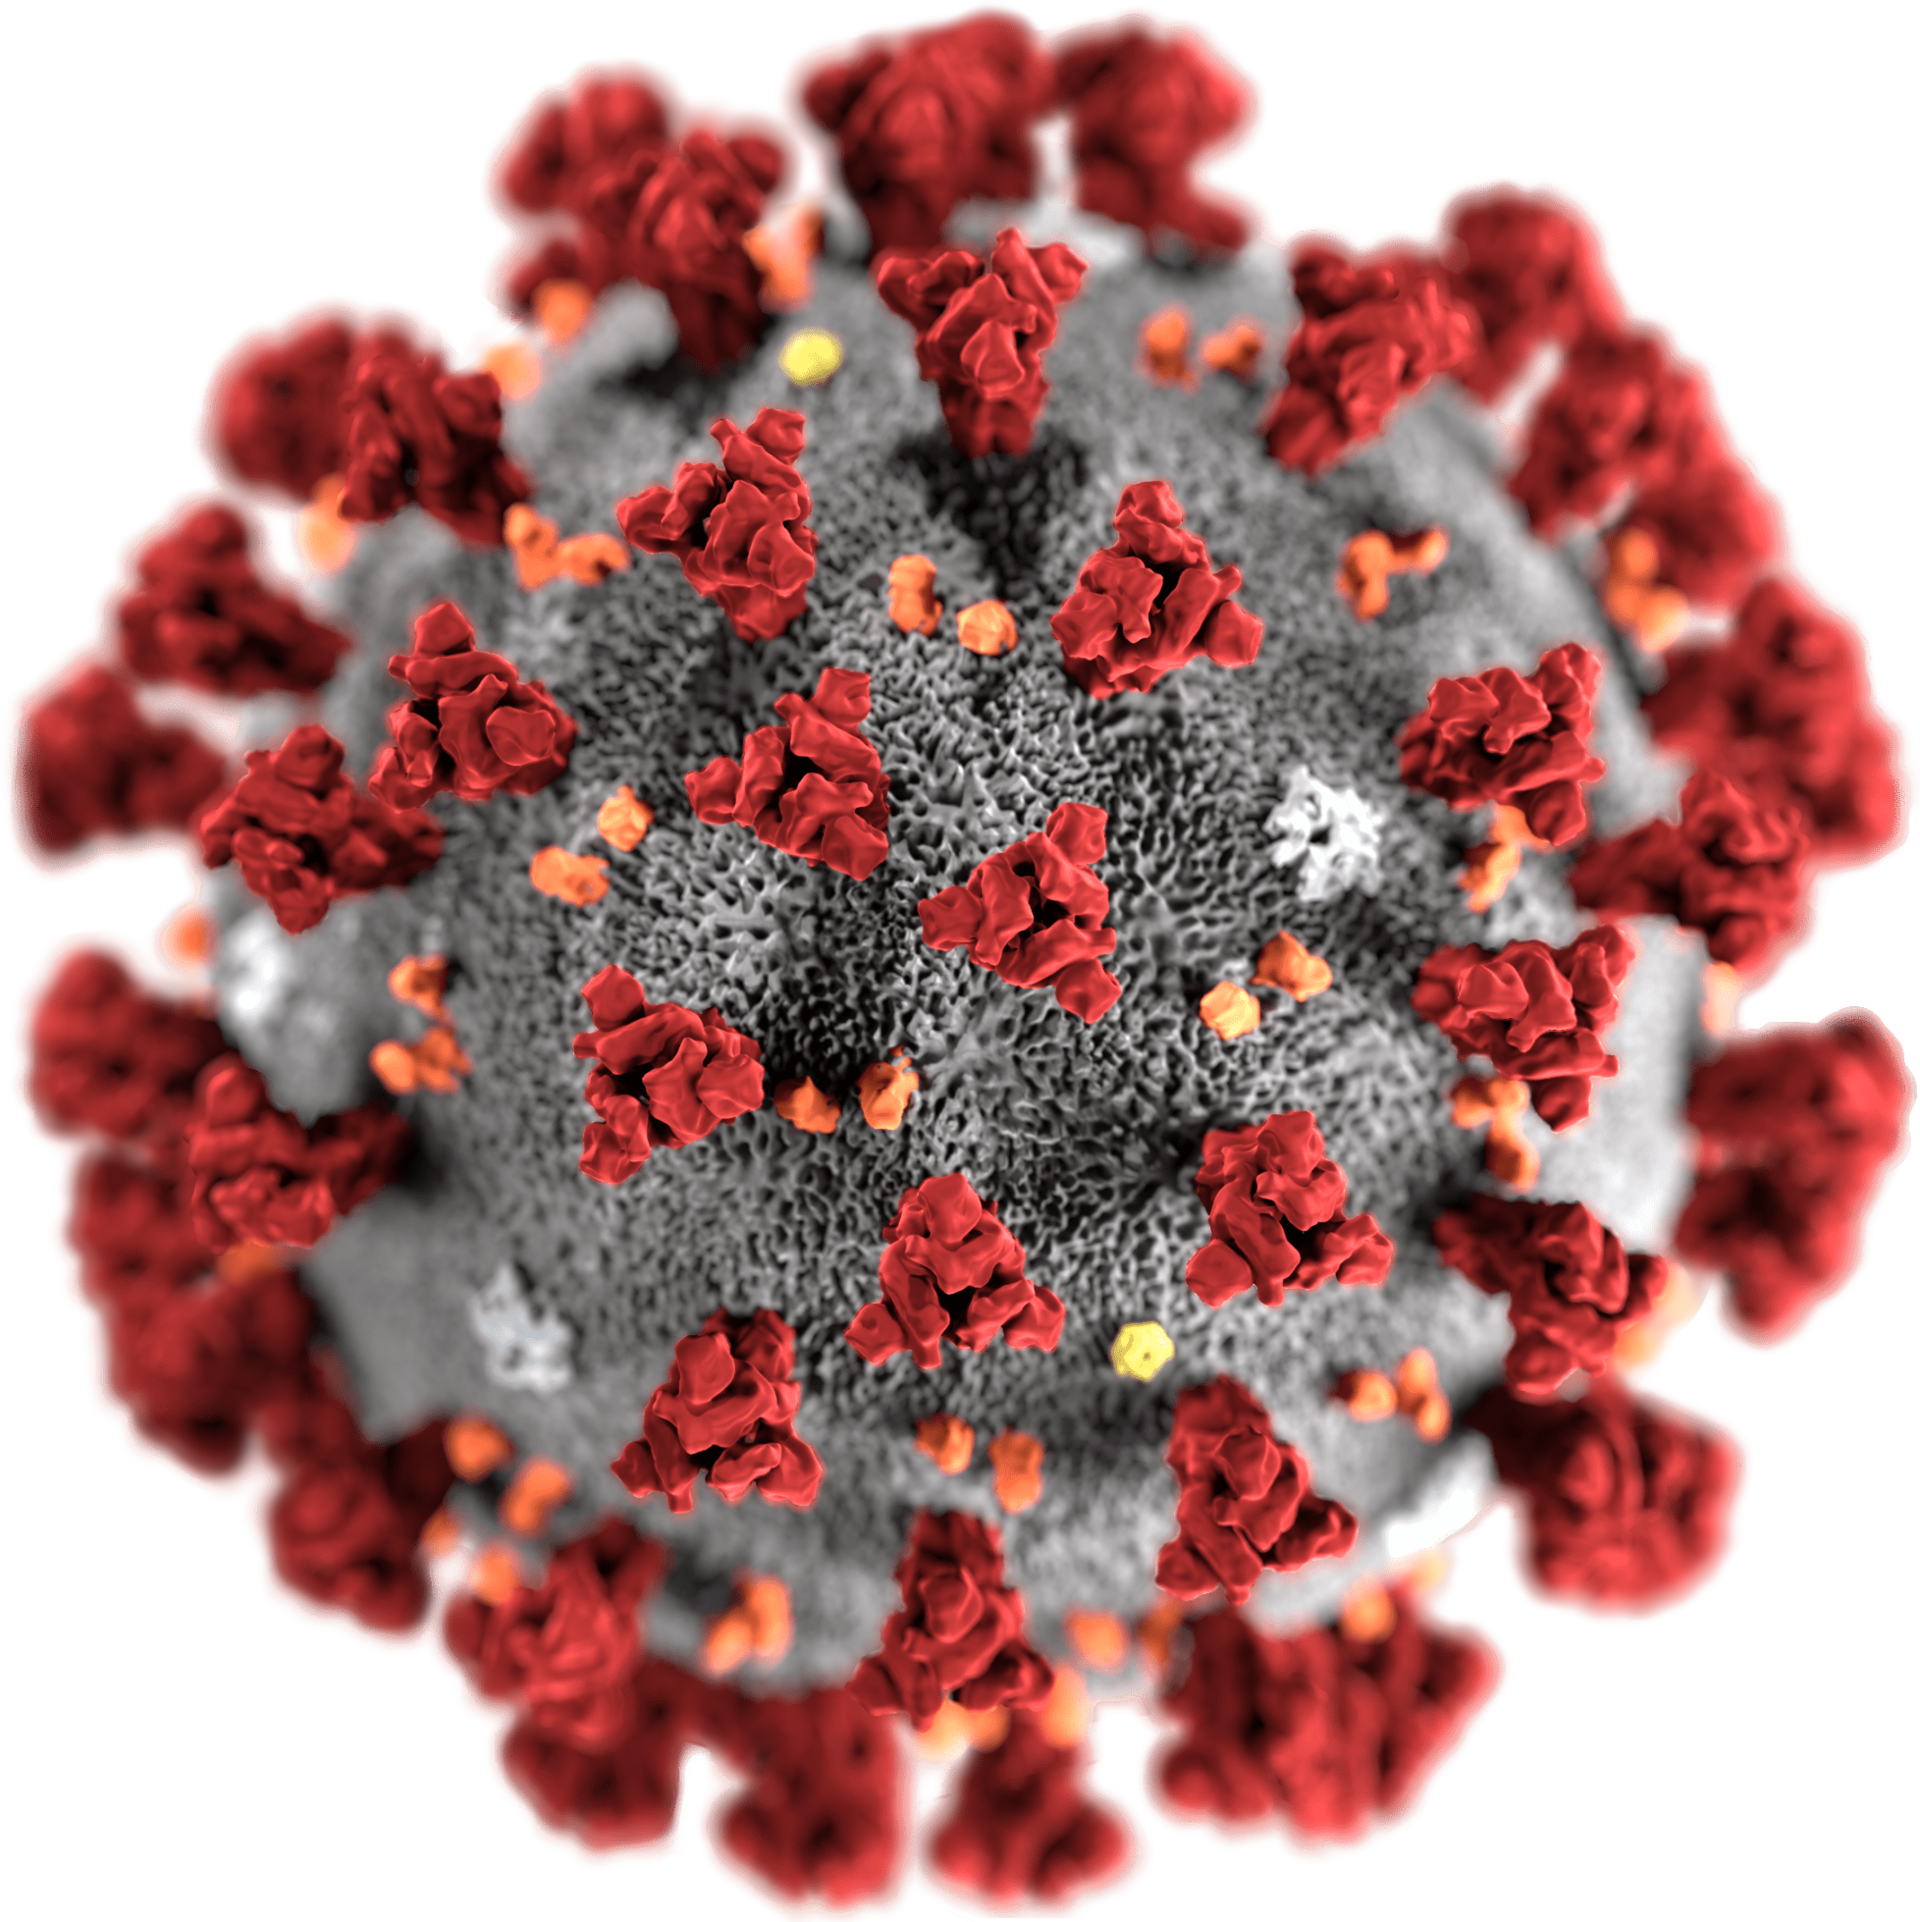
\includegraphics[height = 0.9\textheight]{figures/covid}
\end{center}

\vfill
\tiny{\url{https://phil.cdc.gov/Details.aspx?pid=23312}}
\end{frame}
%%%%%%%%%%%%%%%%%%%%%%%%%%%%%


\frame{\titlepage}


\end{document}
